\sectionSlide{Language popularity}{languages-popularity}{\paperwidth}{t}

\slide{What is the most popular programming language?}{
    \pause
    \centering
    
\includegraphics[height=0.8\paperheight]{it-depends}
}

\slide{C++ users}{
    \begin{columns}
        \begin{column}{0.5\textwidth}
            {\small 
                \begin{table}
                    %\caption{C++ users}
                    \begin{tabular}{|l|r|}
                        \hline \textbf{Date} & \textbf{Estimated users} \\
                        \hline 
                        \hline 1979 & 1 \\
                        \hline 1980 & 16 \\
                        \hline 1981 & 38 \\
                        \hline 1982 & 85 \\
                        \hline 1983 & ??+2 \\
                        \hline 1984 & ??+50 \\
                        \hline 1985 & 500 \\
                        \hline 1986 & 2 000 \\
                        \hline 1987 & 4 000 \\
                        \hline 1988 & 15 000 \\
                        \hline 1989 & 50 000 \\
                        \hline 1990 & 150 000 \\
                        \hline 1991 & 400 000 \\
                        \hline
                    \end{tabular}
            \end{table}}        
        \end{column}
        \begin{column}{0.5\textwidth}
            \pause
            Main users:
            \itemstep{
                \item Bjarne,
                \item Bjarne's colleagues from AT\&T Bell Labs,
                \item universities,
                \item HP, IBM, AT\&T, DEC,
                \item Borland,
                \item Later: Microsoft, Apple,
                \item Now: Google, Facebook
            }
        \end{column}
    \end{columns}
}


\slide{C++ users}{
    \centering 
    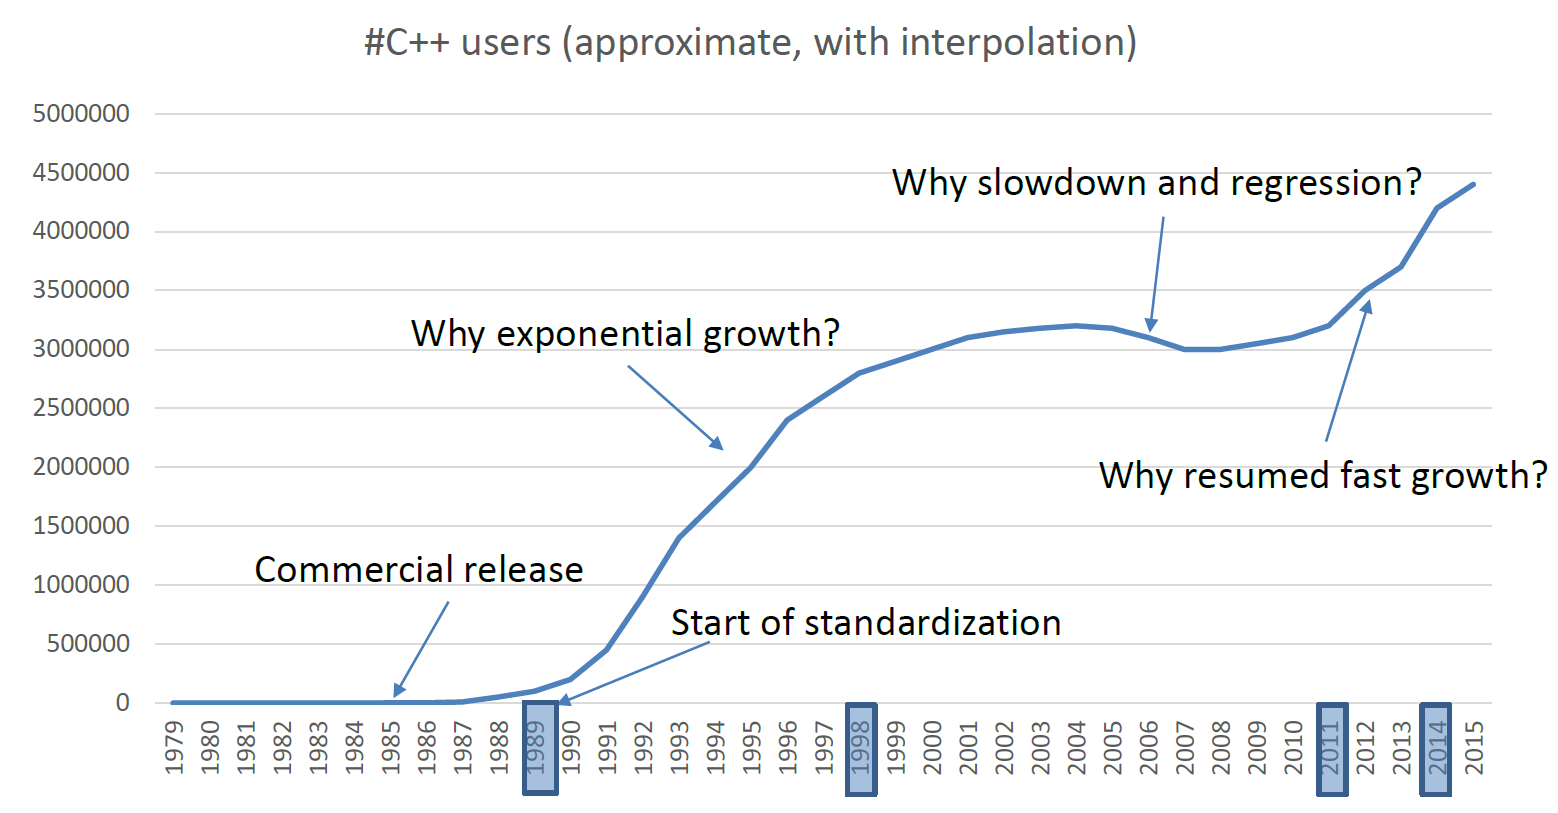
\includegraphics[height=0.78\paperheight]{cpp_users}
    \footnotetext{Bjarne Stroustrup - \textit{The Evolution of C++} - \url{https://www.youtube.com/watch?v=_wzc7a3McOs}}
}


\slide{TIOBE - market share}{
    \only<1>{
        \begin{block}{TIOBE index}
            \textbf{The TIOBE Programming Community} index is an indicator of the popularity of programming languages. The index is updated once a month. Popular search engines such as \textbf{Google, Bing, Yahoo!, Wikipedia, Amazon, YouTube} and \textbf{Baidu} are used to calculate the ratings. Search phrase is \textbf{"language programming"} \\
            Webpage: \url{http://www.tiobe.com/tiobe-index//}
        \end{block}
    }
    \centering
    \includegraphics<2>[height=0.74\paperheight]{tiobe-graph-grey}
    \includegraphics<3>[height=0.74\paperheight]{tiobe-graph}
    \includegraphics<4>[height=0.74\paperheight]{tiobe-array}
}


\slide{PYPL}{
    \only<1>{
        \begin{block}{PYPL index}
            \textbf{The PYPL PopularitY of Programming Language} Index is created by analyzing how often \textbf{language tutorials} are searched on Google: the more a language tutorial is searched, the more popular the language is assumed to be. It is a leading indicator. The raw data comes from \textbf{Google Trends}. \\
            Webpage: \url{http://pypl.github.io/PYPL.html}  
        \end{block}
    }
    \centering 
    \includegraphics<2>[height=0.85\paperheight]{pypl-graph-grey}
    %TODO: Lepiej opisać wykres
    \includegraphics<3>[height=0.85\paperheight]{pypl-graph}
    \includegraphics<4>[height=0.8\paperheight]{pypl-array}
}


\slide{codeeval}{
    \only<1>{
        \begin{block}{codeeval MPCL}
            \textbf{"Most Popular Coding Languages"} is based on hundreds of thousands of data points we've collected by processing over 1,200,000+ \textbf{challenge submissions on codeeval.com} in (now) 26 different programming languages. \\
            Webpage: \url{http://blog.codeeval.com/}  
        \end{block}
    }
    \centering 
    \includegraphics<2>[height=0.83\paperheight]{codeeval2016}
    \includegraphics<3>[height=0.83\paperheight]{codeeval2015}
%    \includegraphics<4>[height=0.34\paperheight]{codeeval2014}
}


\slide{langpop.corger.nl}{
    \centering
    
\includegraphics[height=0.5\paperheight]{github-logo} \vline
    
\includegraphics[height=0.5\paperheight]{stackoverflow-logo} \\
    Webpage: \url{http://langpop.corger.nl/} 
}


\imageSlide{langpop-full}


\slide{Stackoverflow issues}{
    \begin{columns}
    \begin{column}{0.6\textwidth}
        \itemstep{
            \item good programmer == lazy programmer
            \item lazy programmer != good programmer
            \item good programmers do not reinvent the wheel
            \item do job once and never come back here
        }
    \end{column}
    \begin{column}{0.4\textwidth}
        \centering 
        \includegraphics<3->[height=0.8\paperheight]{copying-and-pasting-from-stack-overflow}
    \end{column}
    \end{columns}
}


\slide{C++ is not dead!}{
    \begin{columns}
    \begin{column}{0.6\textwidth}
        \begin{itemize}
            \item In the worst case C++ is on 7th place
            \item In the best case C++ is on 3rd place
            \item C++ is one of the most popular languages!
    		\item Next versions of C++ will be available soon
        \end{itemize}
    \end{column}
    \begin{column}{0.4\textwidth}
        
\includegraphics[height=0.78\paperheight]{bjarne-stroustrup}
    \end{column}
    \end{columns}
}
    
\slide{C++ is not dead!}{
    \begin{columns}
        \begin{column}{0.6\textwidth}
        Future C++:
        \begin{itemize}[<+->]
            \item Type and resource safe
            \item Significantly simpler and clearer code
            \item As fast or faster than anything else
            \item Good at using "modern hardware" (more pipelines, more concurrency)
            \item Significantly faster compilation catching many more errors
        \end{itemize}
    \end{column}
    \begin{column}{0.4\textwidth}
        
\includegraphics[height=0.78\paperheight]{bjarne-stroustrup}
    \end{column}
    \end{columns}
    \footnotetext{Bjarne Stroustrup - \textit{The Evolution of C++} - \url{https://www.youtube.com/watch?v=_wzc7a3McOs}}
}